%% abtex2-modelo-artigo.tex, v-1.9.6 laurocesar
%% Copyright 2012-2016 by abnTeX2 group at http://www.abntex.net.br/ 
%%
%% This work may be distributed and/or modified under the
%% conditions of the LaTeX Project Public License, either version 1.3
%% of this license or (at your option) any later version.
%% The latest version of this license is in
%%   http://www.latex-project.org/lppl.txt
%% and version 1.3 or later is part of all distributions of LaTeX
%% version 2005/12/01 or later.
%%
%% This work has the LPPL maintenance status `maintained'.
%% 
%% The Current Maintainer of this work is the abnTeX2 team, led
%% by Lauro César Araujo. Further information are available on 
%% http://www.abntex.net.br/
%%
%% This work consists of the files abntex2-modelo-artigo.tex and
%% abntex2-modelo-references.bib
%%

% ------------------------------------------------------------------------
% ------------------------------------------------------------------------
% abnTeX2: Modelo de Artigo Acadêmico em conformidade com
% ABNT NBR 6022:2003: Informação e documentação - Artigo em publicação 
% periódica científica impressa - Apresentação
% ------------------------------------------------------------------------
% ------------------------------------------------------------------------

\documentclass[
	% -- opções da classe memoir --
	article,			% indica que é um artigo acadêmico
	11pt,				% tamanho da fonte
	oneside,			% para impressão apenas no recto. Oposto a twoside
	a4paper,			% tamanho do papel. 
	% -- opções da classe abntex2 --
	%chapter=TITLE,		% títulos de capítulos convertidos em letras maiúsculas
	%section=TITLE,		% títulos de seções convertidos em letras maiúsculas
	%subsection=TITLE,	% títulos de subseções convertidos em letras maiúsculas
	%subsubsection=TITLE % títulos de subsubseções convertidos em letras maiúsculas
	% -- opções do pacote babel --
	english,			% idioma adicional para hifenização
	brazil,				% o último idioma é o principal do documento
	sumario=tradicional
	]{abntex2}


% ---
% PACOTES
% ---

% ---
% Pacotes fundamentais 
% ---
\usepackage{lmodern}			% Usa a fonte Latin Modern
\usepackage[T1]{fontenc}		% Selecao de codigos de fonte.
\usepackage[utf8]{inputenc}		% Codificacao do documento (conversão automática dos acentos)
\usepackage{indentfirst}		% Indenta o primeiro parágrafo de cada seção.
\usepackage{nomencl} 			% Lista de simbolos
\usepackage{color}				% Controle das cores
\usepackage{graphicx}			% Inclusão de gráficos
\usepackage{microtype} 			% para melhorias de justificação
% ---
		
% ---
% Pacotes adicionais, usados apenas no âmbito do Modelo Canônico do abnteX2
% ---
\usepackage{lipsum}				% para geração de dummy text
% ---
		
% ---
% Pacotes de citações
% ---
\usepackage[brazilian,hyperpageref]{backref}	 % Paginas com as citações na bibl
\usepackage[alf]{abntex2cite}	% Citações padrão ABNT
% ---

\usepackage{float} 				% para melhorias de justificação

% ---
% Configurações do pacote backref
% Usado sem a opção hyperpageref de backref
\renewcommand{\backrefpagesname}{Citado na(s) página(s):~}
% Texto padrão antes do número das páginas
\renewcommand{\backref}{}
% Define os textos da citação
\renewcommand*{\backrefalt}[4]{
	\ifcase #1 %
		Nenhuma citação no texto.%
	\or
		Citado na página #2.%
	\else
		Citado #1 vezes nas páginas #2.%
	\fi}%
% ---

% ---
% Informações de dados para CAPA e FOLHA DE ROSTO
% ---
\titulo{Offline-first Multidatabase Progressive Web Apps\\ com PouchDB/CouchDB}
\autor{Matheus Dal'Pizzol\thanks{\url{matheusdalpizzol@gmail.com}} \and Anubis Graciela de Moraes Rossetto \thanks{\url{anubisrossetto@gmail.com}}}
\local{Brasil}
\data{2018}
% ---

% ---
% Configurações de aparência do PDF final

% alterando o aspecto da cor azul
\definecolor{blue}{RGB}{41,5,195}

% informações do PDF
\makeatletter
\hypersetup{
     	%pagebackref=true,
		pdftitle={\@title}, 
		pdfauthor={\@author},
    	pdfsubject={Modelo de artigo científico com abnTeX2},
	    pdfcreator={LaTeX with abnTeX2},
		pdfkeywords={abnt}{latex}{abntex}{abntex2}{atigo científico}, 
		colorlinks=true,       		% false: boxed links; true: colored links
    	linkcolor=blue,          	% color of internal links
    	citecolor=blue,        		% color of links to bibliography
    	filecolor=magenta,      		% color of file links
		urlcolor=blue,
		bookmarksdepth=4
}
\makeatother
% --- 

% ---
% compila o indice
% ---
\makeindex
% ---

% ---
% Altera as margens padrões
% ---
\setlrmarginsandblock{3cm}{3cm}{*}
\setulmarginsandblock{3cm}{3cm}{*}
\checkandfixthelayout
% ---

% --- 
% Espaçamentos entre linhas e parágrafos 
% --- 

% O tamanho do parágrafo é dado por:
\setlength{\parindent}{1.3cm}

% Controle do espaçamento entre um parágrafo e outro:
\setlength{\parskip}{0.2cm}  % tente também \onelineskip

% Espaçamento simples
\SingleSpacing

% ----
% Início do documento
% ----
\begin{document}

% Seleciona o idioma do documento (conforme pacotes do babel)
%\selectlanguage{english}
\selectlanguage{brazil}

% Retira espaço extra obsoleto entre as frases.
\frenchspacing 

% ----------------------------------------------------------
% ELEMENTOS PRÉ-TEXTUAIS
% ----------------------------------------------------------

%---
%
% Se desejar escrever o artigo em duas colunas, descomente a linha abaixo
% e a linha com o texto ``FIM DE ARTIGO EM DUAS COLUNAS''.
% \twocolumn[    		% INICIO DE ARTIGO EM DUAS COLUNAS
%
%---
% página de titulo
\maketitle

% resumo em português
\begin{resumoumacoluna}
Este artigo trata do desenvolvimento de \textit{Progressive Web Apps} (PWAs) valendo-se da abordagem \textit{offline-first}. São discutidos os problemas apresentados por aplicativos móveis nativos e as soluções a eles oferecidas pelas PWAs. Discorre-se a respeito dos mecanismos que viabilizam a execução de aplicações Web em um cenário \textit{offline} e sua integração com a interface nativa dos dispositivos móveis, como os Service Workers e o Web App Manifest. A escolha do PouchDB para o armazenamento local das informações é justificada a partir da análise de ferramentas alternativas à tarefa. Estratégias são apresentadas para a sincronização e seguridade de múltiplos bancos de dados para cada usuário em um SGBD CouchDB. Estas estratégias são implementadas em uma aplicação para o auxílio do estudo de instrumentos musicais que tem por objetivo registrar as seções de prática do estudante para análise, referência futura e visualização do progresso do aprendizado do usuário em seu instrumento. Os resultados obtidos são comentados bem como o futuro das PWAs.
\vspace{\onelineskip}

\noindent
\textbf{Palavras-chave}: Progressive Web Apps. Offline-first. PouchDB. CouchDB. Aplicativos Móveis.
\end{resumoumacoluna}

% ]  				% FIM DE ARTIGO EM DUAS COLUNAS
% ---

% ----------------------------------------------------------
% ELEMENTOS TEXTUAIS
% ----------------------------------------------------------
\textual

% ----------------------------------------------------------
% Introdução
% ----------------------------------------------------------
\section*{Introdução}
\addcontentsline{toc}{section}{Introdução}


Russel e Berriman (2015) cunharam o termo \textit{Progressive Web App} (PWA) com o objetivo de denominar websites que “tomaram as vitaminas certas” \cite{russel-2015} para entregar aos usuários uma experiência mais próxima à oferecida por aplicativos móveis nativos enquanto tiram proveito das vantagens clássicas da plataforma Web. Intencionalmente ou não, o conceito de PWA trouxe à luz o que fora, na verdade, a ideia original para a execução de códigos de terceiros em dispositivos móveis quando do lançamento do iPhone pela Apple, em 2007. A visão original da empresa não contemplava a instalação direta de códigos de terceiros no aparelho. O objetivo era que os aplicativos não fossem mais que aplicações web tradicionais, simplesmente apresentadas de forma distinta daquela consagrada nos navegadores \cite{9to5-2011}.

% Problema
Muitos aplicativos nativos para dispositivos móveis destinam-se à solução de problemas e usos pontuais. Em função desta pontualidade, vários desses aplicativos acabam ignorados por apresentarem um custo de oportunidade maior que o de soluções alternativas. De fato, estima-se que 20\% dos usuários interessados em um determinado aplicativo desistem da sua instalação a cada etapa deste processo \cite{cselle-2012} e que 60\% dos aplicativos ofertados em \textit{marketplaces} nunca foram sequer baixados \cite{thygesen-2013}. Em outras palavras, do ponto de vista do usuário, o custo de download e o engajamento exigidos por aplicativos nativos para sua instalação permanente no dispositivo é maior que o de soluções que não envolvam o aplicativo. Ainda, aplicativos nativos não são uma proposição barata do ponto de vista dos desenvolvedores, dado que o suporte à diversas plataformas, dispositivos e versões aumentam seus custos e sua distribuição em \textit{marketplaces} depende de processos burocráticos e tediosos \cite{kumar-2016}. Assim, por facilitar usos descompromissados e pontuais, para a maioria dos casos em que se deseja uma interação que não exija um comprometimento demasiado do usuário, a plataforma Web é mais indicada \cite{lopes-2016}.

O funcionamento centralizado, por sua vez, é um fator frustrante comum a aplicativos móveis nativos e aplicações Web tradicionais, por depender de conexão estável com a Internet e da Nuvem como \textit{Single Source Of Truth} (SSOT) das informações que manipulam.  Não raro, essa característica impede por completo o acesso e a utilização da aplicação. Esses aplicativos também apresentam performance insatisfatória quando operados sob conexões lentas, como 2G e 3G e a observância desses fatores tem profundas implicações no design da camada de comunicação de uma aplicação \cite{prasad-2011}. Ao contrário da ideia difundida de que conectividade ubíqua é uma realidade próxima a ser atingida pelo avanço contínuo em infraestrutura, Alex Feyerke afirma que

\begin{citacao}
	Não tendo conexão de dados com frequência, mesmo nas cidades mais ricas e desenvolvidas do mundo, nos levou a concluir que não, o problema da conectividade/largura de banda não irá simplesmente resolver-se por conta própria em nenhum momento do futuro próximo.” \cite[tradução nossa]{feyerke-2013}
\end{citacao}

% Justificativa
O desenvolvimento de PWAs que mesclem o custo de oportunidade de aplicações Web tradicionais com o engajamento e a imersividade de aplicativos nativos aumenta a atratividade de soluções móveis antes ignoradas por esses fatores e reduz seus custos de distribuição e uso. Por sua vez, a capacitação \textit{offline} de PWAs oferece grandes benefícios e conveniência aos usuários em cenários em que o sinal de Internet seja lento, intermitente ou inexistente \cite{da-14-2017}. O usuário dispõe de uma interface mais rápida, dado que as operações de escrita e leitura são realizadas localmente, reduzindo drasticamente o tempo de resposta. Também há economia de bateria, já que a diminuição de requisições externas reduz os ciclos de processamento e, em cenários de desastre, a aplicação ainda é operável até que a conexão seja restabelecida para a sincronização dos dados com os servidores \cite{holt-2015}.

Tomar consciência desse fato desde o início de um novo projeto é de suma importância devido ao enorme impacto exercido na arquitetura e desenvolvimento das aplicações. Dado que o \textit{workflow  offline-first} é essencialmente diferente do \textit{workflow} de aplicações que assumem a existência permanente de conexões rápidas e confiáveis, o funcionamento \textit{offline-first} dificilmente pode ser implementado incrementalmente, em um momento futuro, sem que haja a reimplementação de grande parte do código \cite{prasad-2011}.

Ademais, é preciso entender que o cenário \textit{offline} não é um erro - como comumente é tratado pelos desenvolvedores -, mas um fato da vida mobile \cite{feyerke-2014} e que uma abordagem \textit{offline-first} é a única maneira de se obter uma experiência ubíqua, ou seja, permitindo a operação da aplicação em qualquer cenário de conectividade \cite{holt-2015}. Ainda, segundo Alex Feyerke

\begin{citacao}
	Nós não podemos continuar construindo aplicativos com o \textit{mindset desktop} de conectividade rápida e permanente, onde uma desconexão temporária ou um serviço lento são tratados como um problema e comunicados como um erro \cite[tradução nossa]{feyerke-2013}
\end{citacao}

% Objetivos
Dessa forma, o presente estudo objetiva o desenvolvimento de uma PWA capaz de operar completamente \textit{offline}, realizando a replicação das informações geridas para a Nuvem apenas quando houver conexão estável com a Internet. Para isso, visa-se realizar o cacheamento do \textit{app shell} utilizando Service Workers; integrar a aplicação à interface do dispositivo do usuário utilizando um Web App Manifest; realizar o armazenamento de informações primariamente no dispositivo do usuário; e realizar a sincronização de informações entre a Nuvem e os dispositivos de usuários.

% Metodologia
Perseguindo esses objetivos, este trabalho apresenta a implementação de uma \textit{Single Page Application} (SPA) com o uso do \textit{framework} de interfaces Vue.js, a biblioteca de componentes Vuetify e o \textit{framework} de aplicação Nuxt.js. A persistência dos dados a nível local se dá com o uso do PouchDB enquanto seu mecanismo de sincronização envia os dados a um servidor CouchDB. Operações restritas a administradores do CouchDB são realizadas através de um servidor intermediário implementado em Express.js.

O presente estudo trata, em sua primeira parte, sobre a visão original para aplicativos móveis, o surgimento do conceito de PWAs, a simulação da experiência nativa em aplicações Web e a capacitação \textit{offline} dessas aplicações. Em seguida, descreve a finalidade da aplicação desenvolvida e como diferentes problemas relacionados à sincronização de múltiplos bancos de dados são abordados. Por fim, apresenta os resultados obtidos durante o desenvolvimento e tece comentários sobre possíveis melhorias e o futuro dos conceitos analisados.


% ----------------------------------------------------------
% Seção de explicações
% ----------------------------------------------------------
\section{Referencial teórico}

Nesta seção são discutidos os conceitos envolvidos no desenvolvimento de PWAs e o resgate da visão original sobre aplicativos móveis. Em seguida, são apresentados os mecanismos que viabilizam a execução de uma aplicação Web \textit{offline} e sua integração com a interface nativa dos dispositivos, bem como a imitação dessas interfaces na plataforma Web. Por fim, são expostas as ideias fundamentais para aplicações \textit{offline-first} e para sincronização de dados distribuídos nessas aplicações utilizando-se PouchDB \cite{pouchdb-2017} e CouchDB \cite{couchdb-2017}.

\subsection{A visão original para aplicativos móveis e as PWAs}

Ao apresentar o iPhone ao mundo, em 2007, Steve Jobs declarou que os desenvolvedores  já, à época,  dispunham de tudo que precisavam para criar aplicativos para o novo dispositivo: bastava valer-se dos padrões modernos da Web. Sua visão original não contemplava a instalação direta de códigos de terceiros no aparelho. O objetivo era que os aplicativos não fossem mais que aplicações Web tradicionais, simplesmente apresentadas de forma distinta daquela consagrada nos navegadores \cite{9to5-2011}.

A afirmação foi ampla e estranhamente ignorada e, em 2008, em resposta aos desenvolvedores, a Apple desviou-se da ideia inicial, dando origem à AppStore \cite{9to5-2011}. Esse acontecimento abriria as portas do prolífero mercado \textit{mobile} dominado pelo iOS e, mais tarde, pelo Android, do Google. Essa reviravolta criou oportunidades na mesma medida em que criou problemas. Como exposto por Alex Russel,

\begin{citacao}
Ao invés de clicar um link para acessar o conteúdo que você está procurando, esses sistemas fazem das lojas os mediadores das aplicações que, por sua vez, mediam e facilitam a descoberta de conteúdo. O processo de “hibridização” gera aplicações que não vivem mais nas ou com as premissas da Web. Como desenvolvemos para todas essas lojas de uma vez só? [...] Como a obrigatoriedade de empacotamento prévio altera seus pressupostos e infraestrutura? Como a indexação para buscas funciona? É uma troca profunda que favorece o suporte \textit{offline} e as lojas em detrimento da rápida iteração e “linkabilidade". \cite[tradução nossa]{russel-2015}
\end{citacao}

Visando alguns desses problemas e aproveitando as melhorias entregues pelas tecnologias Web a partir de 2010, Alex Russel e Frances Berriman definiram o conceito de Progressive Web Apps, enumerando as características necessárias à uma aplicação web para que se mantenham as características da Web enquanto se entrega uma experiência de usuário mais próxima à dos aplicativos nativos. Essas aplicações não são empacotadas e não são distribuídas através de lojas, sendo apenas websites que “tomaram as vitaminas certas” \cite{russel-2015}. As características enumeradas são as seguintes:

\begin{itemize}
	\item
	\textbf{Progressiva:} deve implementar melhoramento progressivo, possibilitando sua operação independentemente das funcionalidades suportadas ou não pelo navegador;
	\item
	\textbf{Responsiva:} deve funcionar igualmente em qualquer tamanho de tela;
	\item
	\textbf{Independente de conectividade:} deve ser melhorada progressivamente com Service Workers para que possa operar \textit{offline};
	\item
	\textbf{App-like:} deve adotar um modelo de aplicação Shell + Conteúdo para criar navegações e interações que simulem as de um aplicativo nativo;
	\item
	\textbf{Atualizada:} deve atualizar-se automática e transparentemente por meio de Service Workers;
	\item
	\textbf{Segura:} devem ser servidas através de HTTPS para garantir a integridade das informações;
	\item
	\textbf{Descobrível:} é identificável através de manifestos W3C permitindo que mecanismos de busca a encontrem;
	\item
	\textbf{Reengajável:} pode acessar as interfaces de reengajamento do sistema operacional, por exemplo, as notificações Push;
	\item
	\textbf{Instalável:} deve poder ser adicionada à \textit{homescreen} do dispositivo através de diálogos do navegador, permitindo que o \textit{app} seja mantido sem a necessidade de uma \textit{app store};
	\item 
	\textbf{Linkável:} deve aproveitar-se do poder social das URLs para compartilhar e ser compartilhada.
\end{itemize}

% ---------------------------------------------------------
% Referencial Teórico: Operação offline com Service Workers
% ---------------------------------------------------------
\subsection{Operação \textit{offline} com Service Workers}

O Service Worker é um tipo específico de Web Worker, tratando-se assim de uma API JavaScript executada à parte do contexto de execução da aplicação principal e, portanto, sem acesso ao Documento Object Model (DOM). Em função disso, os Service Workers são recomendados para a execução de tarefas em \textit{background}, que podem rodar mesmo quando a aplicação estiver \textit{offline}, dando total controle sobre a experiência do usuário aos desenvolvedores \cite{gaunt-2017}. Uma de suas principais características é ser um \textit{proxy} de rede programável, funcionando como um intermediário entre as requisições feitas pela aplicação principal e a rede, permitindo, entre outras coisas, o cacheamento de recursos especificados e endereçáveis por URLs \cite{gaunt-2017}. O esquema é ilustrado na Figura 1.

\begin{figure}[!htb]
	\label{Service Worker}
	\centering
	\caption{Service Worker para busca primária no \textit{cache} e \textit{fallback} para a rede}
	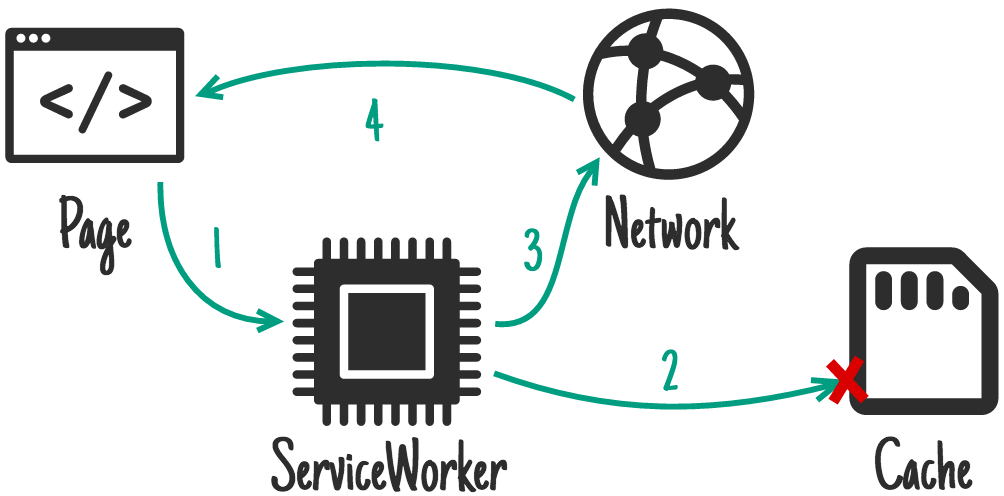
\includegraphics[width=0.6\textwidth]{figures/ss-falling-back-to-network}
	\legend{Fonte: \cite{archibald-2017}}
\end{figure}

Quando 1) requisições feitas pela aplicação são interceptadas pelo Service Worker, 2) é verificada a presença do recurso solicitado no \textit{cache} do navegador. Caso o recurso não exista no \textit{cache}, 3) o Service Worker repassa a requisição para a rede que 4) envia o recurso à aplicação.

Com isso considerado, os Service Workers servem aos propósitos das PWAs em diversos aspectos:

\begin{itemize}
	\item
	Eles permitem que a aplicação seja instalável, podendo efetuar o cacheamento da totalidade do \textit{app shell} (os arquivos estáticos responsáveis pela interface do usuário), permitindo o seu carregamento mesmo em um cenário \textit{offline};
	\item    
	permitem que a aplicação seja automática e transparentemente atualizada, visto que toda vez que a aplicação é acessada, o navegador tenta identificar se o arquivo do Service Worker sofreu alterações, efetuando o download do novo arquivo em caso afirmativo. Entretanto, o antigo Service Worker permanece em execução até que a aplicação seja encerrada e iniciada novamente, quando, então, o novo Service Worker toma o controle;
	\item
	permitem que a aplicação seja reengajável, possibilitando o recebimento de notificações Push, exatamente como as notificações de aplicativos móveis nativos;
	\item
	permitem que a aplicação seja independente de conectividade, possibilitando a sincronização de dados com servidores em segundo plano. Assim, a aplicação pode funcionar \textit{offline}, utilizando a memória do próprio dispositivo para o armazenamento das informações até que haja conexão para que, então, essas informações sejam enviadas para a Nuvem.
\end{itemize}


% ----------------------------------------------------
% Referencial Teórico: Simulação da experiência nativa
% ----------------------------------------------------
\subsection{Simulação da experiência nativa}

Quando o assunto é a experiência do usuário, uma aplicação Web tradicional peca em diversos aspectos se comparada a aplicativos nativos. Para utilizá-la, o usuário precisa abrir o navegador; digitar o endereço do \textit{site}; ver uma tela branca enquanto os recursos são carregados pela rede; ter a barra de navegador ocupando espaço na interface. Todos esses são pequenos detalhes que, por mais insignificantes que pareçam, refletem em frustração e abandono dos usuários. É para sanar esses problemas que, em combinação com os Service Workers, hoje dispomos do manifesto dos aplicativos Web, ou Web App Manifest. Segundo Matt Gaunt e Paul Kinlan,

\begin{citacao}
	O manifesto dos aplicativos Web é um arquivo JSON que permite controlar como o aplicativo Web ou \textit{site} é exibido para o usuário em áreas que normalmente se espera ver aplicativos nativos (por exemplo, a tela inicial de um dispositivo), como definir o que o usuário pode inicializar e o visual durante a inicialização. \cite{gaunt-kinlan-2017}
\end{citacao}

Com algumas poucas propriedades, o Web App Manifest permite que integremos nossa aplicação Web à interface nativa do dispositivo, incluindo a adição de um ícone de inicialização à \textit{homescreen} deste, provendo ao usuário uma experiência praticamente indistinguível daquela fornecida por aplicativos nativos \cite{lopes-2016}.

Para que uma aplicação Web se comporte de maneira visualmente mais próxima de um aplicativo nativo, recomenda-se que ela seja construída na forma de uma Single Page Application (SPA) \cite{lopes-2016}. SPAs são aplicações Web que, através do uso de requisições assíncronas - popularmente conhecidas pela sigla AJAX (Assynchronous JavaScript and XML) -, permitem que novos dados sejam recebidos de servidores Web e apresentados na página já renderizada no navegador do usuário, sem que ele seja obrigado a recarregar a página completamente para visualizar as novas informações. Combinando essa técnica às modernas propriedades CSS (Cascading Style Sheets) de animações e transições, é possível realizar mudanças e trocas suaves entre diferentes componentes da interface gráfica da aplicação, imitando - por vezes de modo muito fiel - a interface gráfica nativa do dispositivo.

Algumas ferramentas auxiliam na obtenção de uma aplicação que disponha de todos esses benefícios, como no causo do Vue.js \cite{vuejs-2017}, Vue-Router \cite{vuerouter-2017} e Vuetify \cite{vuetify-2017}, além do \textit{bundler} Webpack \cite{webpack-2017} e do \textit{framework} de aplicação Nuxt.js \cite{nuxt-2017}.

Enquanto o Vue.js pode ser descrito como um \textit{framework} para a construção de interfaces de usuários, o Vue-Router permite a especificação de componentes Vue.js a serem exibidos quando a URL do navegador corresponder à URL configurada para o componente em questão. Essa configuração pode, então, ser combinada com o empacotamento e separação de código (Code Splitting) realizados pelo Webpack. Assim, cada conjunto de componentes definidos para uma determinada URL pode ser empacotado em um único arquivo JavaScript a ser carregado sob demanda, quando houver a correspondência da URL acessada no navegador. Dessa forma, a obtenção de uma SPA é facilitada. Já o Nuxt.js pode ser descrito como um \textit{framework} de aplicação, mas no fundo, ele consiste de uma série de configurações para Webpack que atendem diversas finalidades, incluindo o preprocessamento de CSS, a compilação de Single File Components do Vue.js, a realização do Code Splitting e a organização do código fonte.

Para completar a simulação da experiência nativa, o Vuetify oferece componentes Vue.js que utilizam o Material Design \cite{material-design-2018}, do Google, a mesma linguagem visual utilizada pelos dispositivos Android, possibilitando a criação de interfaces extremamente fiéis ao visual e à experiência desses dispositivos.

% ---------------------------------------------------------------------------
% Referencial Teórico: Informação offline e distribuída com PouchDB e CouchDB
% ---------------------------------------------------------------------------
\subsection{Informação \textit{offline} e distribuída com PouchDB e CouchDB}

Apesar dos Service Workers possibilitarem a operação \textit{offline} do \textit{app shell} e a sincronização de informações em \textit{background}, eles não são diretamente responsáveis pelo armazenamento local das informações geridas pela aplicação. Além disso, a gestão de informações descentralizadas (replicadas e sincronizadas entre dispositivos e servidores) envolve uma série de problemas complexos e de difícil resolução. Por exemplo, o desenvolvimento de algoritmos de resolução de conflitos e revisões e a prevenção de perda de dados são requisitos que precisam ser implementados desde o início do desenvolvimento da aplicação \cite{martynus-2017}.

Dentre as diversas opções para o armazenamento local de informações estão a Local Storage, a Session Storage e o WebSQL. Todos esses, porém, apresentam problemas como pouco suporte pelos navegadores, limitações graves de espaço em memória, incompatibilidade com Web Workers e funcionamento síncrono bloqueante \cite{osmani-cohen-2017}.

A recomendação atual para o armazenamento local das informações, então, é o IndexedDB \cite{osmani-cohen-2017}. Essa especificação dispõe de bastante espaço na memória, suporta transações, pode ser usada com segurança em diversas abas do navegador simultaneamente e é suportada por todos os navegadores modernos \cite{tabalin-2017}. No entanto, a complexidade de algumas funcionalidades oferecidas pelo IndexedDB implica na complexidade de sua API que, somada à inexistência de suporte ao padrão Promises/A+, dificulta sua utilização pelos desenvolvedores \cite{osmani-2016}. A API do IndexedDB é de tão baixo nível que até mesmo a documentação da Mozilla Developer Network (MDN) alerta os desenvolvedores a esse respeito e recomenda o uso de uma biblioteca \textit{wrapper} para facilitar sua manipulação \cite{smith-2016}.

No entanto, quase a totalidade dessas bibliotecas, à notória exceção do PouchDB, preocupa-se exclusivamente com o armazenamento local, desconsiderando a possível inserção da aplicação em um contexto distribuído e delegando ao desenvolver o tratamento da coesão, replicação e sincronização das bases de dados.

O PouchDB dá diversos passos além da simples facilitação de manipulação do IndexedDB. Abstraindo as diferenças entre o IndexedDB e o WebSQL em uma única API, o PouchDB amplia a capacidade de atuação da base de código, utilizando o IndexedDB como escolha primária de armazenamento e mudando para o WebSQL em navegadores sem suporte ao IndexedDB \cite{brown-2014}.

Sendo uma reimplementação do CouchDB em JavaScript, o PouchDB também implementa o protocolo de replicação do CouchDB, permitindo que as informações salvas mesmo \textit{offline} sejam replicadas e sincronizadas de maneira consistente com a Nuvem, tão logo haja conexão disponível \cite{pouchdb-2017}.

\begin{citacao}
	O super poder do CouchDB é a sincronização. Às vezes eu tento explicar às pessoas dizendo que 'o CouchDB não é um banco de dados, mas um motor de sincronização'. Ele é uma forma eficiente de transferir dados de um lugar a outro, enquanto inteligentemente gerencia conflitos e revisões. É muito semelhante ao Git \cite[tradução nossa]{lawson-2017}.
\end{citacao}

Na Figura 2, podemos verificar a arquitetura de vinculação de dados em quatro vias obtida com o uso do PouchDB e do CouchDB em conjunto, ou 4 Way Data Binding. Os dados obtidos ou apresentados através da interface do navegador são vinculados a um modelo JavaScript que por sua vez referencia os dados persistidos no mecanismo de armazenamento determinado pelo PouchDB para, enfim, serem sincronizados com um servidor CouchDB remoto.

\begin{figure}[H]
	\label{4 Way Data Binding}
	\centering
	\caption{4 Way Data Binding}
	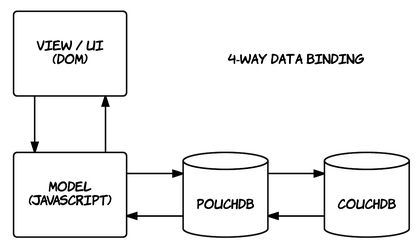
\includegraphics[width=0.6\textwidth]{figures/4way-binding}
	\legend{Fonte: \cite{kumar-nikhil-2016}}
\end{figure}


% -----------
% Metodologia
% -----------
\section{Metodologia}

Esta seção discorre sobre a finalidade da aplicação implementada no estudo dos conceitos apresentados e expõe a forma com que os Service Workers e o Web App Manifest foram à ela adicionados. A subseção sobre segurança e arquitetura apresenta as soluções encontradas para problemas gerados pelas limitações das ferramentas utilizadas, indo desde a criação de bancos de dados isolados para cada usuário, sua autenticação e autorização até a criação programática e sincronização de novos bancos no lado servidor por parte desses usuários. A seção é finalizada com a elucidação do mecanismo utilizado para contornar o problema do limite de requisições paralelas em navegadores Web e manter sincronizados os bancos de dados criados pelos usuários da forma mais transparente possível.

% ------------------------------------
% Metodologia: Finalidade da aplicação
% ------------------------------------
\subsection{Finalidade da aplicação}

A implementação dos conceitos estudados destina-se a uma aplicação para auxílio no estudo de instrumentos musicais. O sistema permite que um usuário registre suas sessões de prática para que, mais tarde, possa visualizar sua evolução. O usuário pode dispor de diversas agendas de treinamento, as quais podem conter diversos exercícios (\textit{licks}). Toda vez que o usuário pratica um exercício, a aplicação registra a duração do exercício, a variação do exercício utilizada - se houver -, a velocidade utilizada em batidas por minuto (BPM) e um \textit{feedback} sobre a execução do exercício para referência futura. No futuro, o usuário deve poder convidar outros usuários para participar de uma mesma agenda de treinamento.

% -----------------------------------------------
% Metodologia: Service Workers e Web App Manifest
% -----------------------------------------------
\subsection{Service Workers e Web App Manifest}

O Nuxt.js facilita a criação de Service Workers e do Web App Manifest, atendendo algumas das exigências das PWAs. Para isso, foi preciso instalar e configurar o módulo do \textit{framework} para PWAs \cite{nuxt-pwa-2018}. O módulo está disponível por gerenciadores de pacotes como o NPM \cite{npm-2017} e o Yarn \cite{yarn-2017}, o que tornou o processo bastante rápido e direto.

O módulo é composto por vários outros submódulos destinados a diferentes finalidades. Um destaque interessante é o Workbox \cite{workbox-2018}, que além de gerar os Service Workers para realizar o cacheamento da aplicação e permitir seu uso \textit{offline}, oferece outros serviços, como o Offline Analytics, que captura os dados de acesso à aplicação mesmo enquanto \textit{offline} e os envia para a conta do Google Analytics quando houver conexão com a Internet.

% ------------------------------------
% Metodologia: Segurança e arquitetura
% ------------------------------------
\subsection{Segurança e arquitetura}

Apesar das facilidades de replicação, o CouchDB oferece alguns desafios quando se trata de segurança e privacidade dos dados. Esses desafios são abordados nesta seção, apresentando possíveis soluções para que os requisitos da aplicação sejam atendidos da maneira mais transparente possível para os usuários, garantindo a integridade e privacidade das suas informações. São explicados os processos de criação de usuários e agendas de treinamento no lado servidor, autenticação e autorização.

\subsubsection{Cadastro de usuários e agendas de treinamento no lado servidor}

Como o CouchDB não oferece nenhum mecanismo de controle de acesso a nível de documentos nem o conceito de coleções, é necessário que cada usuário possua seu próprio banco de dados. Assim, quando um usuário realiza o cadastro no sistema, um novo banco de dados deve ser criado para seu uso exclusivo. O CouchDB facilita esse processo oferecendo a configuração \textit{couch\_peruser}, que realiza a criação automática de um banco de dados com os níveis de acesso corretos toda vez que um novo registro é adicionado ao banco \textit{\_users}.

Efetuado o \textit{login}, o usuário passa a poder criar novas agendas de treinamento a serem gerenciadas. No futuro, cada uma dessas agendas poderá ser compartilhada com outros usuários que poderão visualizar e modificar suas informações. Entretanto, assim como acontece com as informações privadas dos usuários, é necessário que cada agenda possua seu próprio banco de dados a fim de controlar quem pode ou não acessá-la. O problema nesse caso é que, diferentemente do que acontece com o banco de dados criado para o usuário com a opção \textit{couch\_peruser}, o CouchDB não oferece uma opção que realize esse processo automaticamente. Nem o usuário pode realizá-lo pois, como será visto adiante, a criação de bancos de dados é reservada aos administradores do CouchDB.

\subsubsection{Autenticação e autorização}

O CouchDB oferece não só a camada de armazenamento de dados, mas também um serviço RESTful para acesso e manipulação das informações, juntamente com um \textit{framework} de autenticação e autorização \textit{built-in}. O uso desse \textit{framework} é mandatório para que se possa tirar vantagem das funcionalidades de sincronização dessa tecnologia - é preciso que os dispositivos clientes tenham comunicação direta com o servidor  do CouchDB para que mantenham os dados em sincronia. Por outro lado, algumas ações só podem ser realizadas por administradores do CouchDB, como, por exemplo, criar novos bancos de dados ou gerenciar o nível de acesso dos usuários. Como algumas dessas ações terão de ser executadas programaticamente, segundo a demanda dos dispositivos clientes, é necessário um servidor intermediário que detenha acesso de nível administrador ao CouchDB. Esse servidor é implementado utilizando Node.js \cite{node-2017} e o \textit{framework} de HTTP Express.js \cite{express-2017}. A arquitetura é representada na Figura 3.

\begin{figure}[H]
	\centering
	\caption{Arquitetura de autenticação paralela para CouchDB com Express.js}
	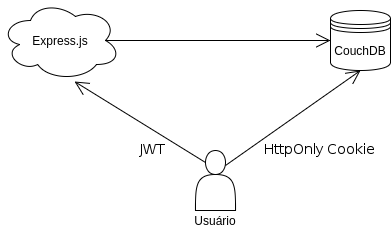
\includegraphics[width=0.6\textwidth]{figures/couchdb-express-proxy-scheme-update}
	\legend{Fonte: Do autor, 2017}
\end{figure}

Nessa arquitetura, enquanto o \textit{framework} de autenticação do CouchDB fornece autenticação por \textit{tokens} baseada em \textit{cookies}, a autenticação no servidor Express.js pode ser realizada através de JSON Web Tokens (JWT) \cite{jwt-2017}. Assim, ao realizar o \textit{login} na aplicação, o dispositivo realiza a requisição de dois \textit{tokens} em paralelo - ambos com os mesmos critérios de expiração -, uma para cada servidor. Mantém-se assim o contato direto do dispositivo do cliente com o servidor CouchDB e possibilita-se a execução programática de operações restritas a administradores através do servidor intermediário. É interessante que não necessariamente ambas as autenticações precisam ser bem sucedidas para que usuário possa utilizar a aplicação, dado que cada um dos \textit{tokens} dá acesso a serviços distintos. Portanto, no caso de um dos serviços encontrar-se \textit{offline}, o usuário simplesmente terá algumas das funções da aplicação temporariamente indisponíveis.

% --------------------------------------------------------
% Metodologia: Sincronização de bancos e compartilhamentos
% --------------------------------------------------------
\subsubsection{Sincronização de agendas de treino e compartilhamentos}

Apesar do protocolo de replicação do CoucDB e o PouchDB ser projetado para a sincronização de informações contidas em um determinado banco de dados, eles não oferecem nenhuma alternativa que sincronize a criação de novos bancos de dados. Além disso, no caso de uso da aplicação proposta, é necessário que as informações de permissões de acesso a determinados bancos de dados também sejam sincronizadas. Como mencionado anteriormente, novos bancos de dados e a modificação das permissões de acesso a esses bancos precisam ser feitas por administradores do CouchDB, portanto, através do servidor Express.js.

A questão torna-se, então: quando realizar essas requisições ao serviço Express.js, visto que, diferentemente do PouchDB, esse serviço não dispõe de um sistema em tempo real? E ainda, como manter uma lista atualizada das contas financeiras de um usuário, dado que esse usuário pode, inclusive, criar novas agendas, deletá-las ou compartilhá-las com outros usuários enquanto estiver \textit{offline}? Ou seja, para que uma nova agenda tenha seu respectivo banco criado no servidor, excluído ou alterado, é necessário ter conhecimento de duas variáveis principais: o \textit{status} da conexão e o \textit{status} da autenticação.

Como a sincronização do banco privado do usuário depende tanto de conexão com a Internet, quanto de autenticação, o melhor momento para a realização dessas operações acontece quando um evento de sincronização bem sucedida é disparado.

Assim, a solução proposta é que cada usuário mantenha uma lista de descrição dessas informações em seu banco privado. Como esse banco pode ser sincronizado normalmente através do PouchDB e apenas o usuário mesmo detém acesso a esse documento, é possível valer-se dos eventos disparados pela \textit{engine} de sincronização e utilizar a lista de descrição remota, sincronizada, para então realizar as operações necessárias. Por exemplo, quando informações alteradas localmente no navegador são sincronizadas com o servidor, a \textit{engine} de sincronização do PouchDB dispara um evento \textit{change} com a propriedade \textit{direction }contendo o valor \textit{push}. A partir disso, pode-se verificar se os documentos da lista de descrição foram modificados e, então, disparar a requisição para o serviço responsável pelas operações de criação de bancos, exclusão de bancos ou modificação de permissões. A Figura 4 apresenta um diagrama desse procedimento.

\begin{figure}[H]
	\centering
	\caption{Diagrama do mecanismo de sincronização de agendas de treino e suas permissões}
	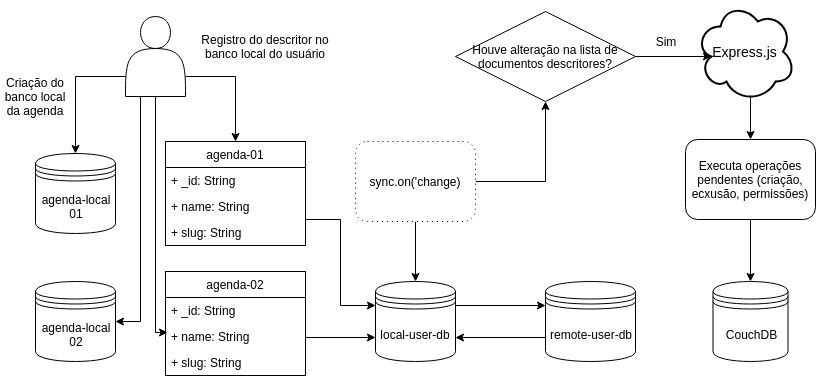
\includegraphics[width=1\textwidth]{figures/riffnailer-sync-database-creation}
	\legend{Fonte: Do autor, 2017}
\end{figure}

É preciso considerar que a requisição em questão pode ser falha e que o serviço intermediário não dispõe de sincronização contínua. Também não é possível assumir que um novo evento \textit{change} contendo um mesmo documento descritor irá ocorrer em um momento futuro. Nesse caso, é preciso informar ao usuário e fornecer meios para que realize essa requisição em outro momento. Algo como “Não foi possível realizar o \textit{backup} dos seus dados. Tentar novamente”.

\subsection{O problema do limite de requisições paralelas em navegadores Web}

Na aplicação proposta, cada agenda de treinamento representa um banco de dados isolado no PouchDB e no CouchDB. Para que esses bancos permaneçam em sincronia, o PouchDB mantém uma requisição aberta entre o dispositivo do usuário e o servidor CouchDB para cada uma das agendas criadas. Porém, os navegadores Web apresentam limites de requisições paralelas a um mesmo \textit{host} que, em geral, é de seis requisições. Se houver mais de seis bancos tentando sincronizar dados com o servidor, qualquer requisição adicional após se atingir o limite será completamente ignorada.

Uma alternativa para a solução desse problema seria o uso de Web Sockets, porém, a manutenção de \textit{sockets} abertos o tempo todo resultaria em consumo desnecessário de bateria, além de carecer de suporte por alguns navegadores. Assim, a solução proposta aqui prevê a sincronização de uma agenda apenas durante o tempo em que ela estiver em uso. Entretanto, essa abordagem traz algumas complicações. Por exemplo, se uma agenda for modificada quando \textit{offline} e não for utilizada quando houver conexão, os seus dados não serão enviados ao servidor CouchDB e, portanto, não serão sincronizados com outros dispositivos.

Para minimizar o problema, foi implementado um mecanismo de \textit{flags} que sinaliza uma agenda como modificada sempre que ela deixar de ser utilizada e tenha sofrido alterações. Essa sinalização é realizada caso o dispositivo esteja \textit{offline} ou caso o usuário não esteja autenticado no momento do término da utilização e a pilha é armazenada na Local Storage. Isso é feito através do \textit{lifecycle hook \textbf{destroyed}}, do Vue.js, que é executado quando o usuário abandona a agenda na GUI (Graphic User Interface) da aplicação. O esquema é ilustrado na Figura 5.

\begin{figure}[H]
	\centering
	\caption{Diagrama do mecanismo de sinalização de modificação \textit{offline} de agendas}
	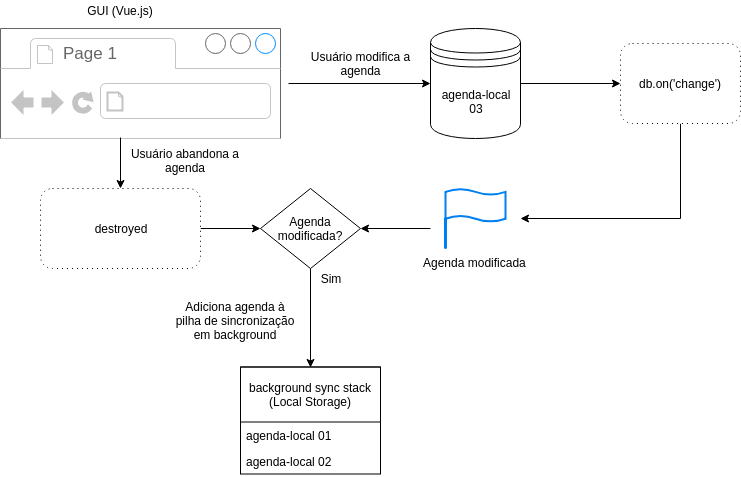
\includegraphics[width=1\textwidth]{figures/riffnailer-schedule-flags}
	\legend{Fonte: Do autor, 2017}
\end{figure}

Após, observam-se alguns eventos que, quando disparados, realizam a sincronização das agendas da pilha em \textit{background}, respeitando o limite de requisições paralelas definido pelo desenvolvedor. A Figura 6 ilustra a ideia.

\begin{figure}[H]
	\centering
	\caption{Diagrama do mecanismo de sincronização em \textit{background}}
	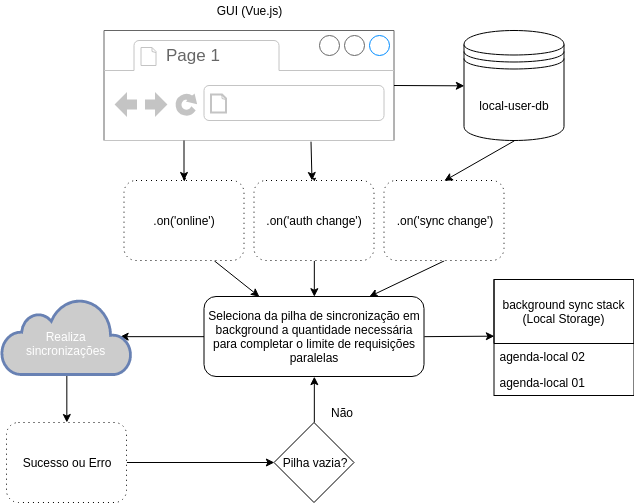
\includegraphics[width=1\textwidth]{figures/riffnailer-schedule-flags-sync}
	\legend{Fonte: Do autor, 2017}
\end{figure}

% ---
% Finaliza a parte no bookmark do PDF, para que se inicie o bookmark na raiz
% ---
\bookmarksetup{startatroot}% 
% ---

\section{Resultados}
\addcontentsline{toc}{section}{Resultados}

O desenvolmineto com Nuxt.js permitiu que algumas características almejadas para a aplicação fossem alcançadas com relativa facilidade. O cacheamento do \textit{app shell} e a integração da interface da aplicação com a interface nativa do dispositivo não necessitaram de mais nada além da instalação do módulo para PWAs do Nuxt.js e sua configuração, já que esse módulo cria o Web App Manifest e os Service Workers necessários aos objetivos mencionados sem que seja preciso escrever esses arquivos desde as suas bases. O Vuetify, por sua vez, tornou possível o desenvolvimento de uma interface gráfica completamente responsiva e extremamente semelhante à interface nativa dos aplicativos para Android. Com isso, a interface da aplicação atendeu à diversas exigências das PWAs, sendo responsiva e \textit{app-like} (através do Vuetify), independente de conectividade, instalável e transparentemente atualizada (através dos Service Workers) e descobrível e linkável (por tirar proveito da plataforma Web).

Com o par PouchDB/CouchDB, a característica \textit{offline-first} foi muito bem incorporada à aplicação, resultando em uma GUI extremamente rápida em que, após o carregamento inicial da aplicação, todas as interações do usuário ocorrem de maneira instantânea. Isso porque nenhuma das operações realizadas pelo usuário depende da realização de requisições HTTP. Por outro lado, não foi possível verificar se houve economia real de bateria dos dispositivos, dado que a aplicação foi executada apenas em ambiente de desenvolvimento por meio de dispositivos conectados via USB e, até o momento, não foi disponibilizada em ambiente de produção.

O mecanismo de sincronização de tarefas restritas a administradores do CouchDB através de um servidor intermediário, descrito na subseção 2.2.3, mostrou-se sólido. Porém, como mencionado, a dependência de uma requisição HTTP convencional para a execução dessas operações, sua suscetibilidade à falhas e a ausência de um mecanismo que tente realizar essas requisições repetidamente até que sejam bem sucedidas, obriga o desenvolvedor a apresentar ao usuário opções para executar essas operações manualmente em caso de falha. Esse fator implica em uma pequena perda de usabilidade, já que operações presumidamente transparentes precisam ser explicitadas aos usuários.

Enfim, apesar de minimizar o problema, a abordagem proposta na subseção 2.3 para sincronização de agendas modificadas quando \textit{offline} serve apenas para o envio de informações ao servidor. Ou seja, um dispositivo ocioso apenas saberá das modificações em uma agenda específica quando esta for acessada na sua própria interface. Porém, esse mecanismo impede que dados deixem de ser enviados ao servidor quando um dispositivo estiver \textit{online} e, tão logo a agenda for utilizada \textit{online} em um dispositivo antes ocioso, os dados estarão disponíveis para sincronização no servidor.

% --------------------
% Considerações finais
% --------------------
\section*{Considerações finais}
\addcontentsline{toc}{section}{Considerações finais}

Atualmente, a abordagem \textit{multidabase} é a única capaz de manter verdadeiramente a privacidade dos dados de um usuário em um sistema CouchDB. Entretanto, essa abordagem acarreta enormes limitações que precisam ser vencidas através de mecanismos de menor estabilidade e coesão em relação ao mecanismo de replicação de documentos do qual usufruem os bancos de dados contidos no CouchDB. Todos esses problemas seriam sanados caso o CouchDB provesse alguma espécie de controle de acesso a nível de documento, o que, sem nenhuma dúvida, diminuiria drasticamente a quantidade de bancos a serem criados e eliminaria a necessidade dos mecanismos descritos nas seções 2.2.3 e 2.3 do presente estudo.

Essa abordagem \textit{multidatabase} também apresenta desafios de arquitetura para a aplicação que devem ser cuidadosamente ponderados. Como cada usuário e cada agenda de treino detém seus bancos de dados isolados, a manutenção de Design Documents precisa atentar ao suporte retroativo e deve ser realizada através da atualização da aplicação nos dispositivos de usuários, já que realizá-la diretamente no servidor CouchDB implicaria na atualização de todos os bancos de dados manualmente ou através de um \textit{script} que varresse todo o SGBD realizando as alterações.

Quando tratamos de performance, a ideia de uma enorme quantidade de bancos de dados pode representar problemas que dependerão do tipo de \textit{hardware} e do sistema operacional utilizados para o servidor CouchDB. Isso se deve ao fato de que requisições ao CouchDB dependem do quão rápido o sistema operacional consegue encontrar, abrir, acessar e fechar os arquivos do banco de dados. Também podem ocorrer problemas em relação à nomenclatura dos bancos já que caracteres especiais pode influenciar a estrutura de pastas do sistema operacional. Por essas razões, torna-se interessante o uso de serviços focados no escalonamento \textit{multidatabase}, como o Cloudant, da IBM, em detrimento de uma instalação nativa do CouchDB.

Por fim, independentemente do uso do par PouchDB/CouchDB ou de qualquer outra ferramenta alternativa dedicada aos objetivos deste estudo, o conceito das PWAs coloca-se como uma alternativa viável e extremamente atrativa aos aplicativos nativos, sendo eles de uso pontual ou não. A distribuição fácil proporcionada pela Web, a ausência de processos de empacotamento em executáveis de instalação dependentes de versões de sistemas operacionais e a proximidade da experiência nativa obtida com as novas tecnologias Web parecem dar início a um movimento em direção à obsolescência dos aplicativos nativos.

% ----------------------------------------------------------
% ELEMENTOS PÓS-TEXTUAIS
% ----------------------------------------------------------
\postextual

% ---
% Título e resumo em língua estrangeira
% ---

% \twocolumn[    		% INICIO DE ARTIGO EM DUAS COLUNAS

% titulo em inglês
\titulo{Offline-first Multidatabase Progressive Web Apps with PouchDB/CouchDB}
\emptythanks
\maketitle

% resumo em português
\renewcommand{\resumoname}{Abstract}
\begin{resumoumacoluna}
 \begin{otherlanguage*}{english}
   This article discusses the development of Progressive Web Apps (PWAs) using
   the offline-first approach. The problems presented by native mobile applications and the solutions offered to them by the PWAs are discussed, as well as the mechanisms that enable the execution of Web applications in an offline scenario and its integration with the native interface of mobile devices, such as the Service Workers and the
   Web App Manifest. The choice of PouchDB for the local storage of information
   is justified by the analysis of alternative tools to the task. Strategies are
   presented for the synchronization and security of multiple databases for
   each user in a CouchDB DBMS (Data Base Management System). These strategies are implemented in an app for the study of musical instruments that keeps track of the students practice sections for analysis, future reference and visualization of their learning progress on the instrument. The obtained results are discussed as well as the future of the PWAs. 

   \vspace{\onelineskip}
 
   \noindent
   \textbf{Keywords}: Progressive Web Apps. Offline-firts. PouchDB. CouchDB. Mobile Apps.
 \end{otherlanguage*}  
\end{resumoumacoluna}

% ]  				% FIM DE ARTIGO EM DUAS COLUNAS
% ---

% ----------------------------------------------------------
% Referências bibliográficas
% ----------------------------------------------------------
\bibliography{pc2-artigo-referencias}

\end{document}
